\documentclass{article}

\usepackage{amsmath}
\usepackage{amssymb}
\usepackage{hyperref}
\usepackage{mathpartir}
\usepackage{palatino}
\usepackage{tikz}


\begin{document}
\begin{enumerate}
\item[1.3.1]
  To show that the epimorphisms in \textbf{Set} are the surjective functions, let $f : A \rightarrow B$ be a surjective function and let $g : B \rightarrow C$ and $h : B \rightarrow C$ be other arrows in \textbf{Set}.
  First, assume both that $g$ and $h$ are equal and that $g \circ f \ne h \circ f$ to derive a contradiction.
  Let $x$ be an element of $A$ such that $g(f(x)) \ne h(f(x))$.
  If $f(x) = y$ we have that $g(y) \ne h(y)$, but this contradicts the assumption that $g$ and $h$ are equal.

  For the converse, assume that $g \circ f = h \circ f$ but that $g \ne h$.
  The first equality states that $\forall x\in A~.~g(f(x)) = h(f(x)) \rightarrow g(y) = h(y)$ if $y = f(x)$.
  Because $f$ is surjective, this derivation shows that $g$ and $h$ agree on all elements of their common domain, thus contradicting the assumption that $g \ne h$.

\item [1.3.2]
  \emph{Goal [1/2]:} $\forall f, g .\,f \mbox{ monic} \wedge g \mbox{ monic} \Rightarrow g \circ f \mbox{ monic}$
  \begin{itemize}
  \item
    Suffices to show: $\forall a, b .\,(g \circ f) \circ a = (g \circ f) \circ b \Rightarrow a = b$
    \\ (by definition $g \circ f$ monic)
  \item
    Assume $(g \circ f) \circ a = (g \circ f) \circ b$
  \item
    $g \circ (f \circ a) = g \circ (f \circ b)$
    \\ (by associativity)
  \item
    $f \circ a = f \circ b$
    \\ (by $g$ monic)
  \item
    Conclude $a = b$
    \\ (by $f$ monic) \qed
  \end{itemize}

\item[]
  \emph{Goal [2/2]:} $\forall f,g .\,g \circ f \mbox{ monic} \Rightarrow f \mbox{ monic}$
  \begin{itemize}
  \item
    Suffices to show: $\forall a, b .\,f \circ a = f \circ b \Rightarrow a = b$
  \item
    Assume $f \circ a = f \circ b$
  \item
    $g \circ (f \circ a) = g \circ (f \circ b)$
    \\ (because $g$ is an arrow)
  \item
    $(g \circ f) \circ a = (g \circ f) \circ b$
    \\ (by associativity)
  \item
    Conclude $a = b$
      \\ (by $g \circ f$ monic) \qed
  \end{itemize}


\item[]
\item[1.3.3]
  \emph{Goal [1/2]:} $\forall f, g .\,f \mbox{ epic} \wedge g \mbox{ epic} \Rightarrow g \circ f \mbox{ epic}$
  \begin{itemize}
  \item
    Suffices to show: $\forall a, b .\,a \circ (g \circ f) = b \circ (g \circ f) \Rightarrow a = b$
    \\ (by definition $g \circ f$ epic)
  \item
    Assume $a \circ (g \circ f) = b \circ (g \circ f)$
  \item
    $(a \circ g) \circ f = (b \circ g) \circ f$
    \\ (by associativity)
  \item
    $a \circ g = b \circ g$
    \\ (by $f$ epic)
  \item
    Conclude $a = b$
    \\ (by $g$ epic) \qed
  \end{itemize}

\item[]
  \emph{Goal [2/2]:} $\forall f,g .\,g \circ f \mbox{ epic} \Rightarrow g \mbox{ epic}$
  \begin{itemize}
  \item
    Suffices to show: $\forall a, b .\,a \circ g = b \circ g \Rightarrow a = b$
  \item
    Assume $a \circ g = b \circ g$
  \item
    $(a \circ g) \circ f = (b \circ g) \circ f$
    \\ (because $f = f$)
  \item
    $a \circ (g \circ f) = b \circ (g \circ f)$
    \\ (by associativity)
  \item
    Conclude $a = b$
      \\ (by $g \circ f$ epic) \qed
  \end{itemize}

\item[]
\item[1.3.4]
  To show that the inverse $f^{-1} : B \rightarrow A$ of an isomorphism $f : A\rightarrow B$ is unique, assume the existence of a function $f^{-1}_2 : B \rightarrow A$ such that $f^{-1} \circ f = id_A = f^{-1}_2 \circ f$ and $f^{-1} \ne f^{-1}_2$.
  Let $y$ be an element of $B$ such that $f^{-1}(b) \ne f^{-1}_2(b)$, and let $x$ be the preimage of $b$ in $f$.
  Then we have $f^{-1}(f(x)) \ne f^{-1}_2(f(x)) \Rightarrow f^{-1}(y) \ne f^{-1}_2(y) \rightarrow x_1 \ne x_2$ for unequal elements $x_1,x_2 \in A$.
  However, if $x_1 \ne x_2$ then either (or both) of $x_1$ and $x_2$ cannot equal $x$.
  If $x_i = x$ does not hold, then the ``inverse'' function was incorrect; an isomorphism preserves identity.

\item[]
\item[1.3.5]
  We show that if $f : A \rightarrow B$ and $g : B \rightarrow C$ are isomorphisms then $g \circ f$ is an isomorphism with $f^{-1} \circ g^{-1}$ as its inverse.

  First, define objects $A$, $B$, and $C$.
  \begin{center}
    \begin{tikzpicture}
      \node (1) {$A$};
      \node[right of=1,xshift=1cm] (2) {$B$};
      \node[right of=2,xshift=1cm] (3) {$C$};
    \end{tikzpicture}
  \end{center}

  By definition, we have arrows $f : A \rightarrow B$ and $f^{-1} : B \rightarrow A$ such that $f^{-1} \circ f = id_A$.
  \begin{center}
    \begin{tikzpicture}
      \node (1) {$A$};
      \node[right of=1,xshift=1cm] (2) {$B$};
      \node[right of=2,xshift=1cm] (3) {$C$};

      \draw[->] (1) edge[bend left] node[above] {$f$} (2);
      \draw[->] (2) edge[bend left] node[below] {$f^{-1}$} (1);
    \end{tikzpicture}
  \end{center}

  Likewise, we have $g : B \rightarrow C$ and $g^{-1} : C \rightarrow B$ such that $g^{-1} \circ g = id_B$.
  \begin{center}
    \begin{tikzpicture}
      \node (1) {$A$};
      \node[right of=1,xshift=1cm] (2) {$B$};
      \node[right of=2,xshift=1cm] (3) {$C$};

      \draw[->] (2) edge[bend left] node[above] {$g$} (3);
      \draw[->] (3) edge[bend left] node[below] {$g^{-1}$} (2);
    \end{tikzpicture}
  \end{center}

  Together, these arrows yield the diagram:
  \begin{center}
    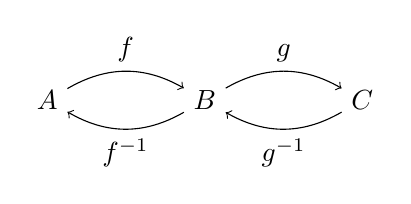
\begin{tikzpicture}
      \node (1) {$A$};
      \node[right of=1,xshift=1cm] (2) {$B$};
      \node[right of=2,xshift=1cm] (3) {$C$};

      \draw[->] (1) edge[bend left] node[above] {$f$} (2);
      \draw[->] (2) edge[bend left] node[below] {$f^{-1}$} (1);
      \draw[->] (2) edge[bend left] node[above] {$g$} (3);
      \draw[->] (3) edge[bend left] node[below] {$g^{-1}$} (2);
    \end{tikzpicture}
  \end{center}

  From which it is clear that $(f^{-1} \circ g^{-1}) \circ (g \circ f) = id_A$.

\item[]
\item[1.3.6] The category $\textbf{2}$ has an arrow, $f$, that is both a monomorphism and an epimorphism but not an isomorphism. 
  \begin{center}
  \begin{tikzpicture}[node distance=2cm, auto]
  \node (A) {$A$};
  \node (B) [right of=A] {$B$};
  \draw[->] (A) to node {$f$} (B);
  \end{tikzpicture}
  \end{center}
  This holds because of the limited number of compositions we can make. 
  Ignoring composition of identities, there are only two possibilities: $id_A;\ f$ and $f;\ id_B$. 
  Yet there is no arrow $f^{-1}: B \rightarrow A$, so $f$ is not an isomorphism.
\end{enumerate}
\end{document}
